\section{Description du mode de ventilation}

\begin{frame}{Courbe pression-temps typique}
	\centering
		\begin{tikzpicture}
		\begin{axis}[
				width=\textwidth,
				height=0.7\textheight,
				enlarge y limits=upper,
				enlarge x limits=false,
				xmax=8,
				xlabel=Temps (sec.),
				ylabel=Pression (hPa)
				]

			\addplot table [y=Pao ] {dat/simvent1.dat};
		\end{axis}
	\end{tikzpicture}

\end{frame}

\begin{frame}{Haute et basse fréquence}
	\tikzstyle{plage}=[<->, shorten <=0.25mm, shorten >=0.25mm]

\tikzset{
	zoomline/.style={
		opacity=.5,
		dotted
	},
}

\def\zstart{7.2}
\def\zend{7.8}
\def\istart{2}
\def\tic{2}
\def\pstart{7.365}
\def\tip{0.059}

\tikzsetnextfilename{lfhf}
\begin{tikzpicture}
	\begin{groupplot}[
			group style={
				group size=1 by 2,
				y descriptions at=edge left,
				xlabels at=edge bottom
			},
			ylabel=Pression (hPa),
			xlabel=Temps (s),
			max space between ticks=40,
			height= 0.42\textheight,
			enlarge y limits={value=0.9, upper},
			enlarge x limits=false
		]

		\nextgroupplot[
			width=\textwidth]

		\addplot table[x=time, y=Pao] {dat/simvent1.dat};


		\coordinate (PSO) at (axis cs:\zstart,0);
		\coordinate (PSE) at (axis cs:\zend,0);
		\coordinate (PNO) at (axis cs:\zstart,\pgfkeysvalueof{/pgfplots/ymax});
		\coordinate (PNE) at (axis cs:\zend,\pgfkeysvalueof{/pgfplots/ymax});

		\draw [plage](axis cs:\istart,45) -- (axis cs:\istart + \tic, 45) node[midway, above] {Inspi.};
		\draw [plage](axis cs:\istart + \tic,45) -- (axis cs:\istart + 2*\tic, 45) node[midway, above] {Expi.};

		\draw [dashed] 
		(axis cs: \istart,\pgfkeysvalueof{/pgfplots/ymax}) -- (axis cs:\istart,0)
	 	(axis cs: \istart + \tic,\pgfkeysvalueof{/pgfplots/ymax}) -- (axis cs:\istart + \tic,0)
		(axis cs: \istart + 2 *\tic,\pgfkeysvalueof{/pgfplots/ymax}) -- (axis cs:\istart + 2*\tic,0);

		\draw [zoomline] (PSO) rectangle (PNE);


		\nextgroupplot[
				max space between ticks=80,
				width=0.75\textwidth,
				axis background/.style={fill=gray!15, opacity=0.8},
				]

		\addplot +[
			restrict x to domain=\zstart:\zend
			] table[x=time, y=Pao] {dat/simvent1.dat};

		\coordinate (ZNO) at (axis cs:\zstart,\pgfkeysvalueof{/pgfplots/ymax});
		\coordinate (ZNE) at (axis cs:\zend,\pgfkeysvalueof{/pgfplots/ymax});
		\coordinate (ZSO) at (axis cs:\zstart,\pgfkeysvalueof{/pgfplots/ymin});
		\coordinate (ZSE) at (axis cs:\zend,\pgfkeysvalueof{/pgfplots/ymin});


		\draw [dashed] 
		(axis cs: \pstart,\pgfkeysvalueof{/pgfplots/ymax}) -- (axis cs:\pstart,0)
		(axis cs: \pstart + \tip,\pgfkeysvalueof{/pgfplots/ymax}) -- (axis cs:\pstart + \tip,0)
		(axis cs: \pstart + 2 *\tip,\pgfkeysvalueof{/pgfplots/ymax}) -- (axis cs:\pstart + 2*\tip,0);

		\draw [plage] (axis cs:\pstart,45) -- (axis cs:\pstart + \tip, 45) node[midway, above] {Insp.};
		\draw [plage](axis cs:\pstart + \tip,45) -- (axis cs:\pstart + 2*\tip, 45) node[midway, above] {Exp.};

	\end{groupplot}

	\begin{scope}[
			%on background layer
		]
		\fill [opacity=0.075](PSO) rectangle (PNE);
		\draw [zoomline](ZNO) -- (PNO) (PNE) -- (ZNE) ;
		\draw [zoomline](ZSO) -- (PSO) (PSE) -- (ZSE) ;
	\end{scope}

\end{tikzpicture}

\end{frame}

\begin{frame}{Échanges gazeux en ventilation haute fréquence}
	\tikzset{
	bronche/.style={
		double distance=1cm,
		double=pink,
		thick
	}
}
	\begin{columns}[T, onlytextwidth]
		\column{0.4\textwidth}
		\begin{block}{Débit laminailre}
	\begin{tikzpicture}[
			every pin/.style={
				font=\scriptsize
			},
			]
		\draw [
			bronche,
		]
		(.5,0) -- (.5, -3.35) node [midway, minimum width=1.1cm,
		pin=0:{(Ceci est une bronche !)}] {};
		%\draw (0,0) -- (0,-3.25);
		%\draw (1,0) -- (1,-3.25);
		\shade[
			left color   = bleuclairchum,
			right color  = bleuclairchum,
			middle color = marinechum,
			rounded corners
		]
		(0,0) -- (0.5,-3) --  (1,0);
		\node [white] at(0.5, -1) {$\downarrow$};
		\node [white] at(0.25, -.5) {$\downarrow$};
		\node [white] at(0.75, -.5) {$\downarrow$};
		\node [white] at(0.5, -2) {$\downarrow$};
	\end{tikzpicture}
	\end{block}

		\column{0.4\textwidth}
		\begin{block}{Débit turbulent}
	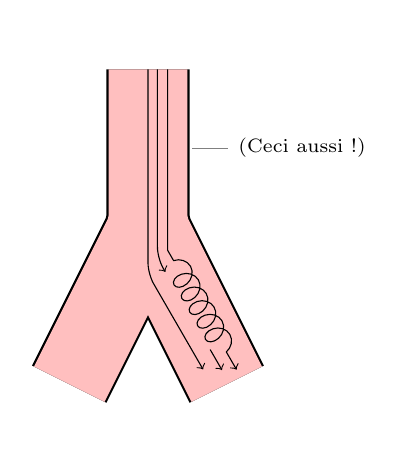
\begin{tikzpicture}[
			every pin/.style={
				font=\scriptsize
			},
			]
			\draw [
				bronche,
				rounded corners,
			] (0,0) -- (0,-2) node [midway, minimum width=1.1cm, pin=0:{(Ceci
			aussi !)}] {}--
			++(1, -2) (0,0) -- (0,-2) -- ++(-1,-2);
			\draw [->, rounded corners] (0,0) -- ++(-90:2.6) -- ++(-60:1.4) ;
			\draw [->, rounded corners] (.12,0) -- ++(-90:2.4) -- ++(-60:.2) ;
			\draw [
				->,
				decoration={
					coil,
					amplitude=1.5mm,
					aspect=.8,
					segment length=2mm,
					pre length=1.5mm,
					post length=1.5mm,
				}
			]  
			(.25,0) -- ++(-90:2.3) decorate {-- ++(-60:1.75)} ;
			\draw [->, rounded corners] (.12,0) ++(-90:2.4) ++(-60:1.34) --
			++(-60:.3);
	\end{tikzpicture}
		\end{block}
	\end{columns}

\end{frame}

\begin{frame}{Le phasitron}
	\begin{columns}
		\column{0.60\textwidth}
		\tikzsetnextfilename{phasitron}
\begin{tikzpicture}[
		every node/.style={
			align=center,
			font=\footnotesize
		}
]
\pic [name=Phasitron, scale=0.4] {phasitron};
	\node [left=2mm] at (Phasitron-Pt) {Patient $\leftrightarrow$};
	\node [below=2mm] at (Phasitron-E) {$\downarrow$\\Expiration};
	\node [below=2mm, align=center] at (Phasitron-A) {$\uparrow$\\Appel d'air};
	\node [right=2mm] at (Phasitron-S) {$\leftarrow$ Pressurisation};
	%\node [below=2mm, anchor=north east] at (Phasitron-M) {Monitorage};
\end{tikzpicture}

		\only<2>{\centering
\tikzsetnextfilename{dilution}
\begin{tikzpicture}
\begin{axis}[
		xlabel=Pression \tiny{($cmH_2O$)},
		ylabel=Ratio $\frac{Appel\ d'air}{Air\ inject \acute{e}}$,
		width=0.5\textwidth,
		%height={},
		%title=Ratio d'appel d'air théorique du phasitron,
		font=\small,
		schoolbook
]
	\addplot +[very thick] coordinates {(0,5) (40,0)};
\end{axis}
\end{tikzpicture}
%\footcite{Percussionairecorporation2009}
}

		\column{0.35\textwidth}
		\tikzset{
			flow/.style={
				structure, 
				->, 
			},
			small flow/.style={
				flow,
				line width=.2mm,
			},
			mid flow/.style={
				flow,
				line width=.5mm,
			},
			big flow/.style={
				flow,
				line width=1mm,
			},
}
%\begin{columns}
%	\column{0.5\textwidth}
	\begin{block}{Insuflation}
		\vspace{.25cm}
	\begin{tikzpicture}[
			scale=.45,
			every node/.style={transform shape},
			]

	\pic [name=P, draw=black!50, fill=gray!10] {phasitron-coupe};
	\pic {venturi-avance};

	\path (P-S) -- (P-Pt) 
		node [pos=0.32] (Junction) {}
		coordinate [pos=0.15] (Diafragm)
		;

	\draw [small flow] (P-S) ++(3mm,0) to (Diafragm);
	\draw [small flow, shorten <=1mm] (Diafragm) to (Junction);

	\draw [
		mid flow,
		out=90, 
		in=-45,
		shorten >=1mm
	] (P-A) ++ (0, -3mm)  to (Junction);

	\draw [big flow] (Junction)  to (P-Pt);
	
\end{tikzpicture}
	\end{block}

%%%%%%%%%%%%%%%%%%%%%%%%%%%%%%%%%%%%%%%%%%%%%%%%%%%%%%%%%5
%%%%%%%%%%%%%%%%%%%%%%%%%%%%%%%%%%%%%%%%%%%%%%%%%%%%%%%%%5

	%\column{0.5\textwidth}
	\begin{block}{Expiration}
		\vspace{.25cm}

	\begin{tikzpicture}[
			scale=.45,
			every node/.style={transform shape}
			]

	\pic [name=P, draw=black!50, fill=gray!10] {phasitron-coupe};
	\pic {venturi-recule};

		\draw [
			big flow,
			out=0, 
			in=90, 
			looseness=1.8,
			] ([yshift=-4mm]P-Pt) to (P-E);

\end{tikzpicture}
	\end{block}
%\end{columns}

	\end{columns}
\end{frame}

\begin{frame}{Pression alvéolaire}
	\centering
	\begin{tikzpicture}
\begin{axis}[
	width=\textwidth,
	height=0.7\textheight,
	enlarge y limits=upper,
	enlarge x limits=false,
	xmax=8,
	xlabel=Temps (sec.),
	ylabel=Pression (hPa),
	legend=true,
	legend image post style={mark=none}
]

	\addplot table [mark=none, y=Pao ] {dat/simvent1.dat};
\addlegendentry{Pcirc}
	\addplot table [mark=none, y=Palv ] {dat/simvent1.dat};
\addlegendentry{Palv}

\end{axis}
\end{tikzpicture}

\end{frame}

\begin{frame}{Pression motrice}
	\centering
	\newcommand{\pexp}{5}
\newcommand{\pins}{18}
\newcommand{\arrpos}{1.57}
\def\aShift{4.1cm}

\begin{tikzpicture}
	\begin{axis} [
			height=0.80\textheight,
			width=0.75\textwidth,
			extra y ticks={\pexp, \pins},
			extra y tick labels={$P_{ins. moy.}$, $P_{exp. moy.}$},
			xtick={0,2,4},
			ytick={0,30},
			axis x line=bottom,
			axis y line=middle,
			enlarge y limits={0.2, upper},
			extra y tick style={
				grid=major, 
			},
			major grid style={
			}
		]

		\addplot +[
			restrict x to domain=0:4,
			]table[x=time, y=Pao] {dat/simvent1.dat};

		\coordinate (A) at (axis cs:\arrpos,\pexp);
		\coordinate (B) at (axis cs:\arrpos,\pins);
	\end{axis}
		\draw [
			very thick,
			->,
			shorten >=1mm, 
			shorten <=1mm, 
			font=\small
		](A) -- (B) node [pos=0.6, left=3mm, rounded corners, thin]{$P_{motrice}$};

\end{tikzpicture}

\end{frame}

%\begin{frame}
%	\frametitle{Caractéristiques du mode de ventilation}
%	\begin{itemize}
%		\item Haute et basse fréquence simultanée
%		\item Adaptation dynamique aux changements de mécanique pulmonaire
%		\item Respiration spontanée permise
%		\item Expiration passive
%	\end{itemize}
%\end{frame}
